\documentclass[12pt,a4paper,titlepage,oneside,BCOR1cm]{scrreprt}



\usepackage[utf8]{inputenc}
\usepackage{graphicx}
\graphicspath{ {images/} } 
\usepackage[final]{pdfpages}
\usepackage{fancyhdr}
\usepackage[pdfpagelabels]{hyperref}
\usepackage{amsmath,amstext,amssymb}
\usepackage{rotating}
\usepackage{afterpage}

\usepackage[english,german]{babel}
\usepackage{csquotes}

\usepackage[style=reading,sorting=nty,backend=bibtex]{biblatex}
\addbibresource{bibliography.bib}

%\bibliographystyle{gerunsrt} % Literaturangaben nach Auftreten sortieren %{gerplain}

\date{\today}
\author{Robin Maximilian Ruth}
\title{Bachelorthesis proposal -- Sparked}

\begin{document}
\thispagestyle{empty}

\begin{figure}[htbp]
\centering
 \begin{minipage}[b]{41 mm}
   
\includegraphics[width=40 mm]{./figures/DAI_Logo.png}
 \end{minipage}
\end{figure}

~\vspace{0.5cm}

\begin{center}
\begin{Huge}
Technische Universitaet Berlin\\
\vspace{1mm}
\end{Huge}{\Large Fakultaet IV - Elektrotechnik und Informatik\\
Fachgebiet AOT\\
Prof. Dr. Sahin Albayrak}\\

\vspace{26mm}
\begin{LARGE}
Bachelorthesis proposal\\
\end{LARGE}
\vspace{8mm}
\begin{LARGE}
Sparked, an intuitive user interface for the automated machine learning project CODA\\
\end{LARGE}
\vspace{3 cm}
Robin Ruth\\
Matrikel--Nummer 316672\\
\vspace{1cm}
\begin{tabular}{lll}
    \textbf{Betreuer} & Researcher Christian Geissler & Dipl.-Inform. ABC\\
\end{tabular}

\end{center}

\tableofcontents
\thispagestyle{empty}


\pagenumbering{arabic}
\chapter{Motivation}
With the ongoing digitalisation and the generation of big data in most aspects of society, data driven approaches to every day problems become more and more viable. One way to evaluate these large datasets is with an machine learning approach. Machine learning, though powerfull is not a wonder box. Not every machine learning approach is applicable for every problem and not every algorithm will perform in reasonable time on every data.

You need a lot of intimate knowledge and intuition about machine learning algorithms to select a good approach to your given problem. Knowledge and intuition that is only developed in few experts. Even then, to optimize for a given problem still requires a lot of trial and error, as most of the time the best hyperparameter settings can only be found by trial and error.

To find a way to automate this process, DAI-Labor (Distributed Artifical Intelligence) and GTARC (German Turkish Advanced Research Center for ICT) have started CODA, a fundamental resarch project in algorithm selection and hyperparameter optimisation. (PROJEKTSTECKBRIEF!)

With this project, nicknamed Sparked, we create an interface to the CODA project, allowing machine learning enthusiasts and specialists to use the developed solutions and giving the CODA team an interface to demonstrate CODAs capabilities.

As such we will provide a user interface that is usable in demonstrations and can be used by persons with a background in machine learning without prior training. As such a focus is set on a clean workflow, good user guidance and a visual appealing display.

\chapter{Objective}
The overall objectiv of Sparked is to create a web application and a supporting backend to interface with the CODA backend.

To develop Sparked an architecture has to be chosen. This includes which technologies will be used in the development process. 

The architecture has to support several criteria:
\begin{itemize}
  \item Demonstration startup
  
  It should be easy to spin up a clean Sparked instance with empty databases for demonstration purposes. Sensible defaults should apply, to make such an instance immediatelly usable even by an untrained individual.

  \item Configurability

  Changing the CODA Backend should be possible without recompile.

  \item Docker deployment

  Sparked has to run in docker containers on a linux system.

\end{itemize}

Some common characteristics of web applications are not relevant in this project:
\begin{itemize}
  \item Useraccounts

  All Users will operate on the same data. There will not be any useraccounts. Any data uploaded to Sparked is visible to all other users.
  \item Login

  The UI will be open and not contain any login features or any other form of access controll.
\end{itemize}

Coda will run on a seperate machine, connected via a bus system (Kafka). Kafka access is not part of the Sparked project. An encapsulation library (Java) will be provided.

Sparked contains several workflows:
\begin{itemize}
  \item Order creation

  An order can be created. This includes the selection of all values needed to create an order. classifier, metric, test dataset and validation method with their respective parameters.

  After an order is created, it will be split in tasks and put into a queue for processing. This includes persisting them to have a keep them in data on restart.

  \item Order overview

  View all orders, with their tasks and allows them to be paused or continued if not finished. A Sparked instance will connect to a single backend. 

  \item Order evaluation
  
  Open and display order and task results.
\end{itemize}

It is not possible to access several CODA backends at the same time. 


\chapter{Work packages}

The project is roughly seperated in 3 parts:
\begin{itemize}
  \item Architecture
  \item Development
  \item Evaluation
\end{itemize}


\section{Architecture}
\begin{itemize}
  \item UX Design
  \item UI Design
  \item Technolology evaluations
  \item System architecture
\end{itemize}  

\section{Development}
\begin{itemize}
  \item Let the user create an orders and save them
  \item Create the tasks needed to evaluate an order
  \item Display all orders, show their progress and stop, pause and unpause them
  \item Receive and display the results of an order
  \item Configuration page
  \item Bugfixing
\end{itemize}
\section{Evaluation}
  \begin{itemize}
    \item Find people to interview
    \item Create the interview questionair
    \item Hold the interview
    \item Evaluate the given statements
  \end{itemize}

\hspace*{-1.5in}
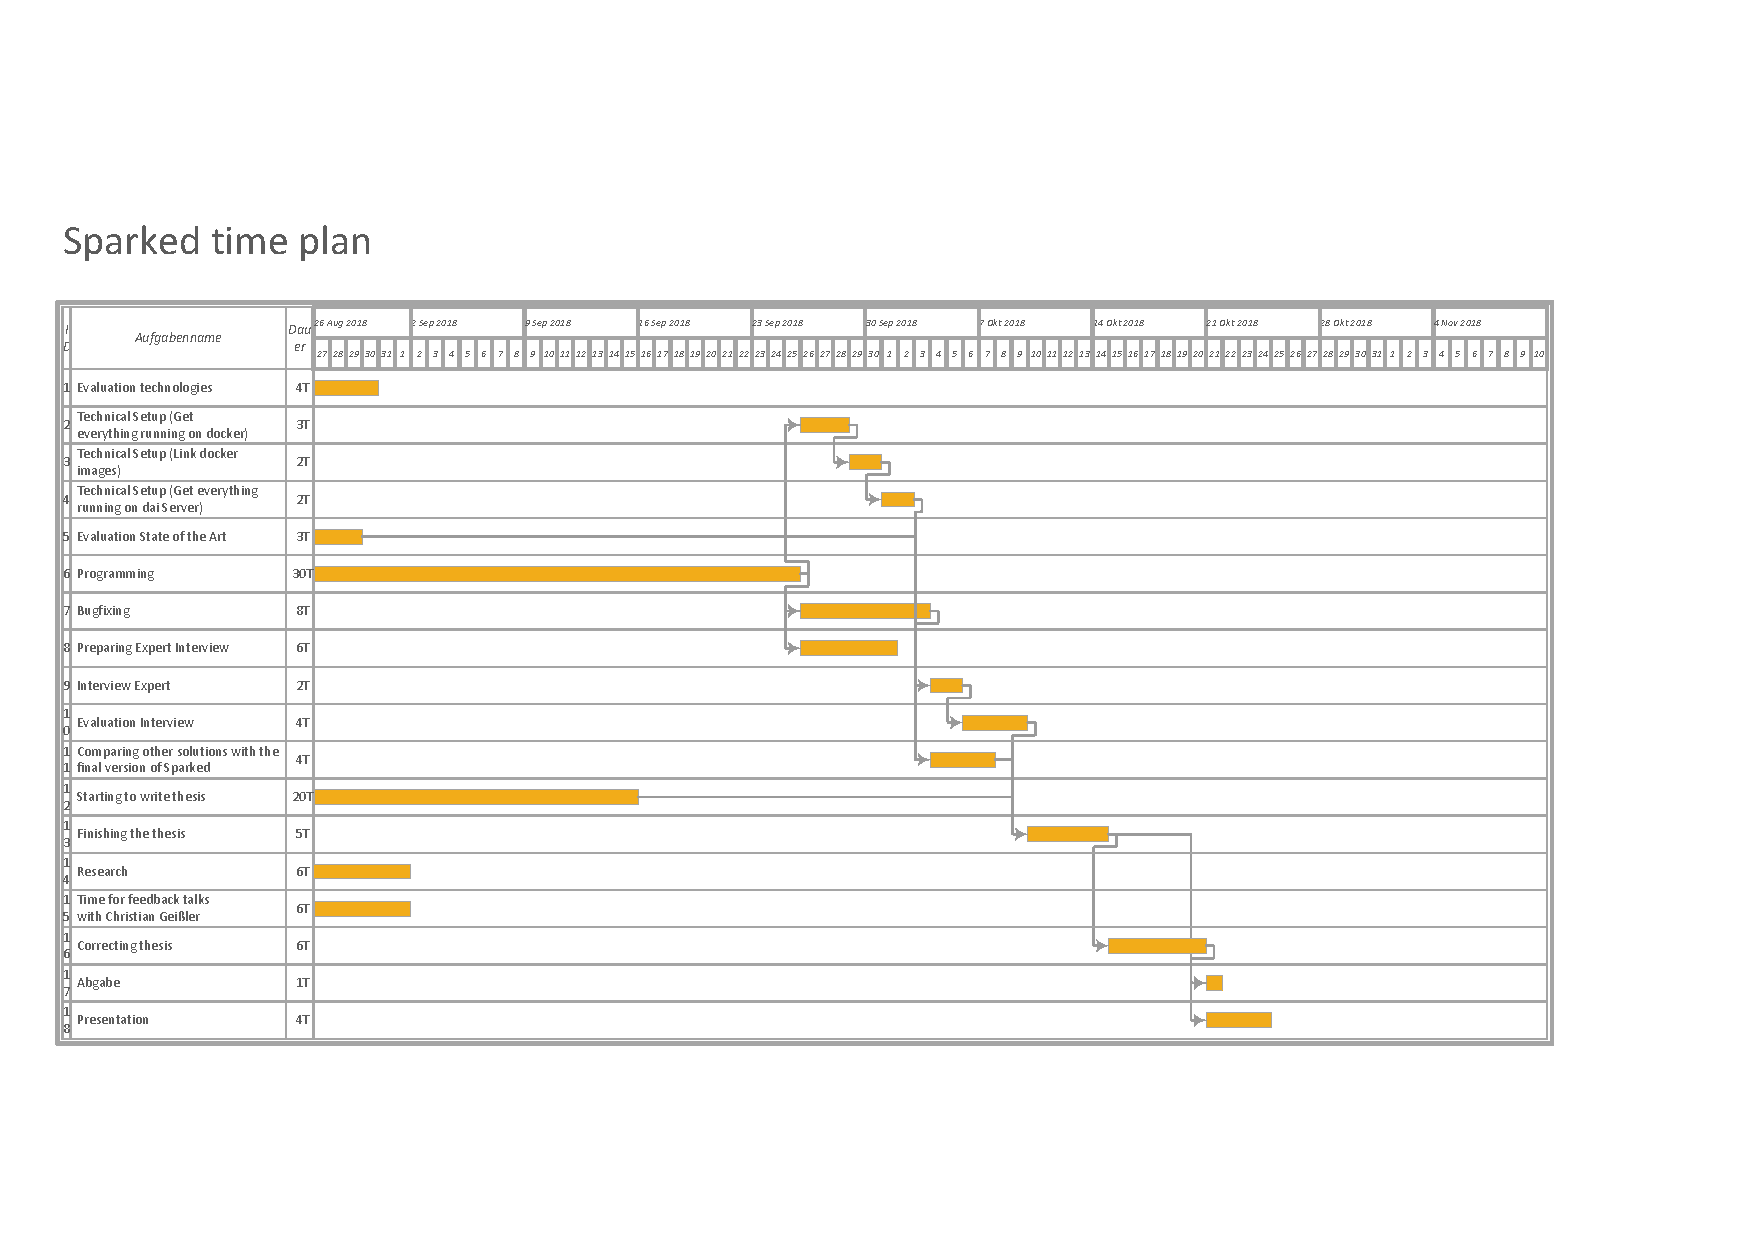
\includegraphics[width=\paperwidth]{gantt-proposal-2.pdf}

\chapter{Organizational}
\begin{itemize}
\item Language of this Bachelorthesis is english.
\item The thesis will be written with pdflatex.
\item Choosing programming languages and technologies are not defined and part of the development process.
\item Supervisors is Christian Geißler
\item Evaluators are Prof. Dr. Albayrak and Prof. Kao \cite{inproceedings}
\end{itemize}

\chapter{Appendix}

\afterpage{
\thispagestyle{empty}
\vspace*{-1.2in}
\hspace*{-1.5in}
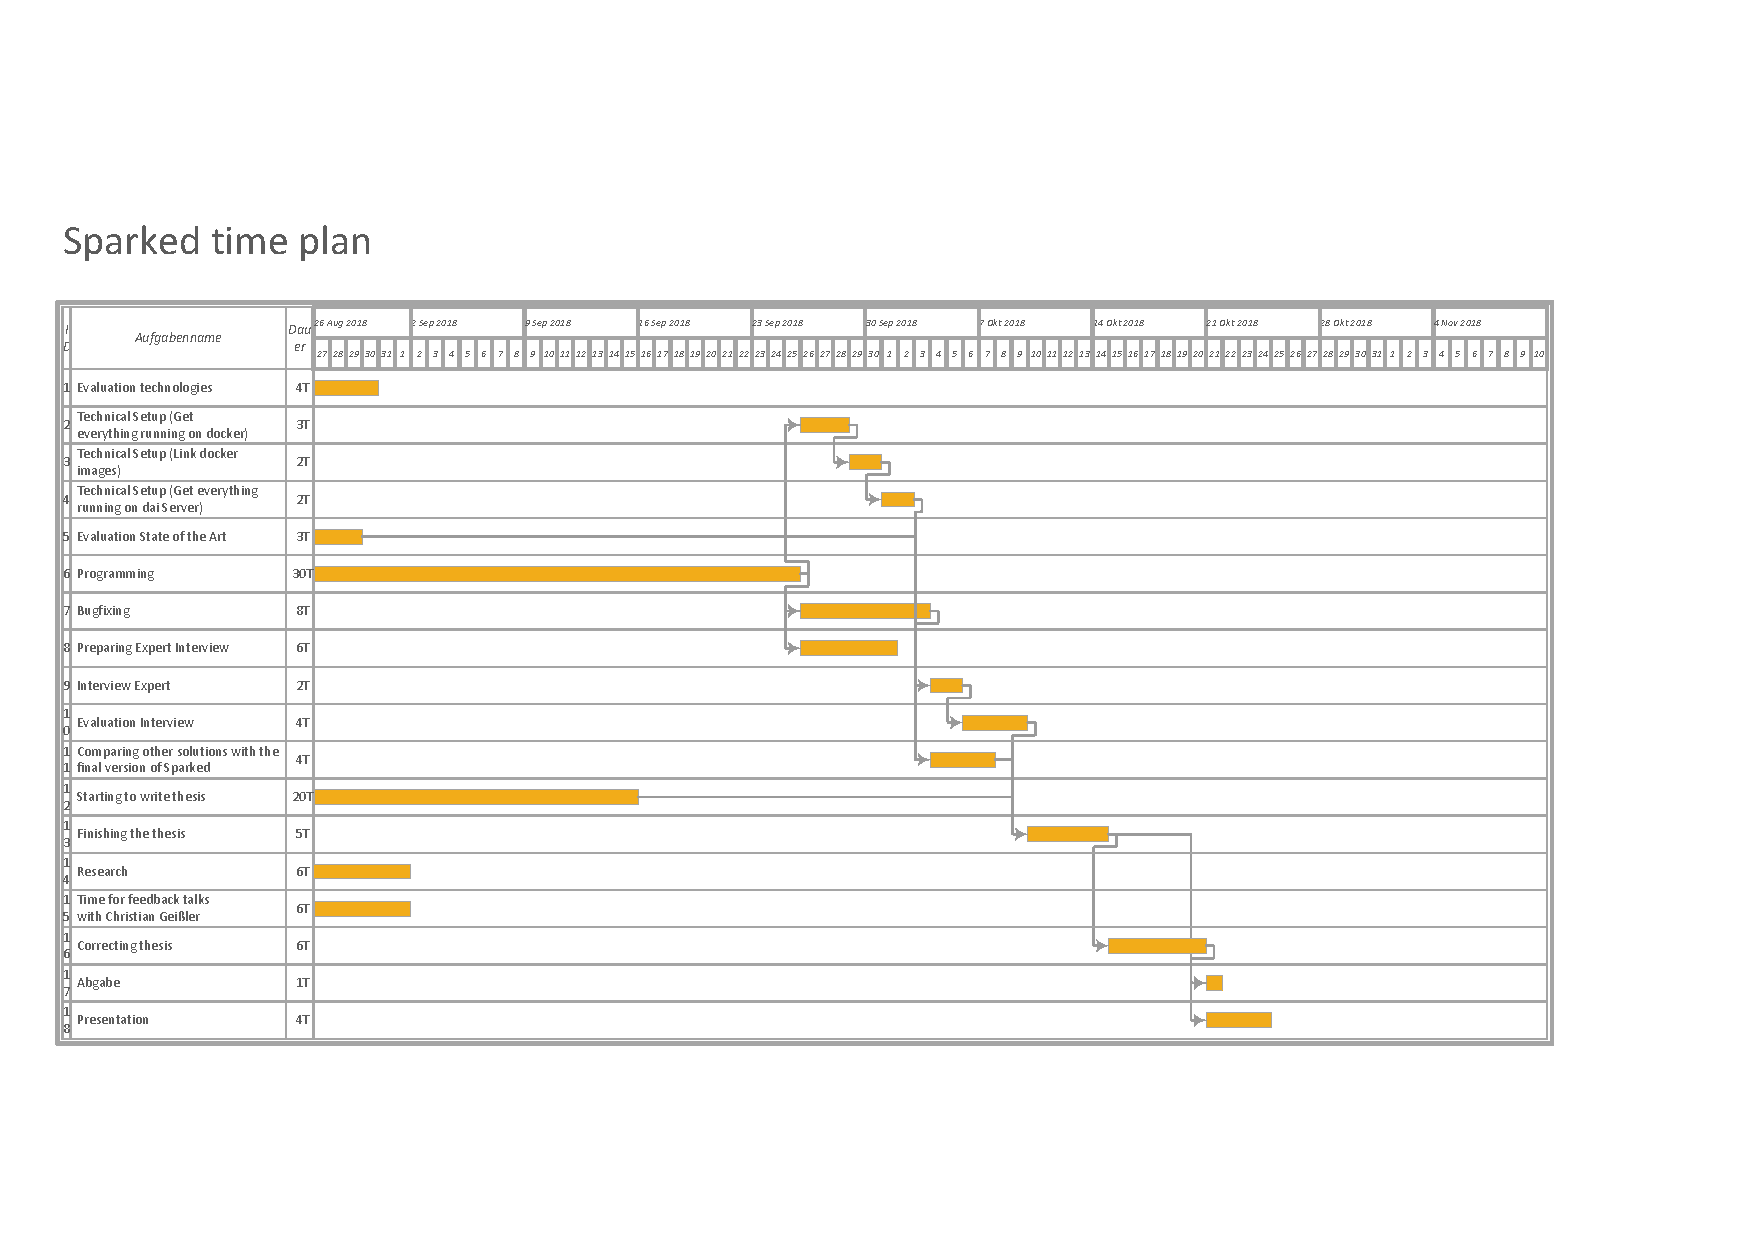
\includegraphics[angle=90, height=\paperheight]{gantt-proposal-2.pdf}
}
\newpage

\nocite{*}

\printbibliography

\end{document}
